%   ##
%
%   Band VIII, 3 N.~??A10.1
%   Signatur/Tex-Datei: LH_35_09_15_006-007
%   RK-Nr. 41152 [Teil 1]
%   Überschrift: Tentaminum de chordarum tensione scheda prima
%   Datierung: 1680.12.10
%   WZ: (keins)
%.  SZ: (keins)
%.  Bilddateien (PDF): LH_35_09_15_006-007_d1; LH_35_09_15_006-007_d2; LH_35_09_15_006-007_d3 (insgesamt drei) 
%
%
\begin{ledgroupsized}[r]{120mm}
\footnotesize
\pstart
\noindent\textbf{Überlieferung:}
\pend
\end{ledgroupsized}
\begin{ledgroupsized}[r]{114mm}
\footnotesize
\pstart \parindent -6mm
\makebox[6mm][l]{\textit{L}}%
Aufzeichnung: LH~XXXV~9,~15~Bl.~6\textendash7.
Ein Bogen 4\textsuperscript{o}.
Vier einspaltig beschriebene Seiten.
Im Kopf von Bl.~6~r\textsuperscript{o} gestrichene Zeile von Leibnizens Hand:
\edlabel{LH_35_09_15_006r_Ueberlieferung-1}\textit{Si com\-pres\-sio\protect\index{Sachverzeichnis}{compressio}
fit per extru\-sionem\protect\index{Sachverzeichnis}{extrusio}
subtilis materiae\protect\index{Sachverzeichnis}{materia subtilis}
est expressio}.\protect\index{Sachverzeichnis}{expressio}\edlabel{LH_35_09_15_006r_Ueberlieferung-2}
% Kein Wasserzeichen.
\pend
\end{ledgroupsized}
%
%
\vspace{4mm}% !!!! Vorläufig geändert !!!!
%
%
\count\Bfootins=1000
\count\Afootins=1000
\count\Cfootins=1000
%
%
\pstart%
\normalsize%
\noindent%
%
% % % %    ACHTUNG GETRIXT: Folgende Cfootnote bezieht sich auf die Überlieferung
\edtext{}{%
{\xxref{LH_35_09_15_006r_Ueberlieferung-1}{LH_35_09_15_006r_Ueberlieferung-2}}% compressio
{\lemma{\textit{Si} \lbrack...\rbrack\ \textit{expressio}}\Cfootnote{%
Vgl. \cite{00044}H.~\textsc{Fabri}, \textit{Physica}, tract. I, lib. II, prop. 18 (Bd. I, Lyon 1669, S.~53b\textendash54a).}}}%
%
%
\lbrack6~r\textsuperscript{o}\rbrack % Blatt 6r
%
\pend%
% \vspace*{-0.5em}%
% Überschrift
\pstart%
\centering%
\edtext{Tentaminum de Chordarum tensione%
\protect\index{Sachverzeichnis}{tentamen}%
\protect\index{Sachverzeichnis}{tensio chordae}}{%
\lemma{Tentaminum}\Bfootnote{%
\hspace{-0,5mm}de Chordarum tensione
\textit{erg.~L}}}
%
Scheda\protect\index{Sachverzeichnis}{scheda}
\edtext{prima.
10 Xb. 1680}{% \edlabel{LH_35_09_15_006r_titel-1}
\lemma{prima}\Bfootnote{%
\textit{(1)}~in q
\textit{(2)}~. 10 Xb. 1680%
~\textit{L}}}%
\pend%
\vspace{0.5em}%
%
\pstart%
\centering%
De chordis
\edlabel{LH_35_09_15_006r_Anfang-1}tensis\protect\index{Sachverzeichnis}{chorda tensa}
\edtext{}{{\xxref{LH_35_09_15_006r_Anfang-1}{LH_35_09_15_006r_Anfang-2}}%
{\lemma{tensis}\Bfootnote{%
\textit{(1)}~\textso{Chordae tensae quaelibet pars aeque tensa est,} id est a toto separata ac sibi relicta sese contraheret in ea ratione in qua se contrahit tota. Nam Aeque tensa sunt
\textit{(2)}~Ut intelligatur \lbrack...\rbrack\ autem chordae
\textit{(a)}~aequales et similes
\textit{(b)}~aeque
\textit{(aa)}~longe
\textit{(bb)}~longae et crassae eiusdemque materiae
\textit{(aaa)}~aeque tensae sunt,
\textit{(bbb)}~sunt aeque tensae, si
\textit{(aaaa)}~eodem modo pulsatae se eodem
\textit{(aaaaa)}~modo
\textit{(bbbbb)}~tempore restituant
\textit{(bbbb)}~simul eodem \lbrack...\rbrack\ simul restituant.
\textit{(aaaaa)}~Item si
\textit{(bbbbb)}~Hinc chordae alicujus
\textit{(aaaaa-a)}~duae
\textit{(bbbbb-b)}~plures partes \lbrack...\rbrack\ simul restituuntur
\textit{(aaaaa-aa)}~eaedemque partes etiam materiae ejusdem sunt longitudinisque et crassitiei.
\textit{(bbbbb-bb)}~. Suppono autem \lbrack...\rbrack\ et crassitiei.
\textit{(aaaaa-aaa)}~Sed quid
\textit{(bbbbb-bbb)}~Si ead
\textit{(ccccc-ccc)}~Sed ejusdem chordae partes inaequales an aeque sint tensae quaeri potest.
\textit{(aaaaa-aaaa)}~Hoc judicari
\textit{(bbbbb-bbbb)}~Quod ut dignoscatur
\textit{(ddddd-ddd)}~\textbar~Unde sequitur \lbrack...\rbrack\ auget tensionem. \textit{erg.}~\textbar\ Sed ut \lbrack...\rbrack\ ejus causa.%
~\textit{L}}}}%
\pend%
% \vspace*{0.5em}%
%
\pstart%
\noindent%
Ut intelligatur % \edlabel{LH_35_09_15_006r_titel-2}
distincte quid sit\textso{ tensio,}\protect\index{Sachverzeichnis}{tensio}
inquirendum est quae aeque aut magis minusque tensa dicantur.
Duae autem chordae aeque longae et crassae
eiusdemque\protect\index{Sachverzeichnis}{materia chordae} materiae sunt aeque tensae,
si simul eodem modo pulsatae\protect\index{Sachverzeichnis}{chorda pulsata}
se simul restituant.\protect\index{Sachverzeichnis}{restitutio chordae}
Hinc chordae alicujus plures partes aequales aeque sunt tensae,\protect\index{Sachverzeichnis}{chorda tensa}
nam tota simul restituitur,
itaque et partes illae simul restituuntur.\protect\index{Sachverzeichnis}{restitutio chordae}
Suppono autem partes illas esse similes
seu materiae\protect\index{Sachverzeichnis}{materia chordae} ejusdem
et crassitiei.\protect\index{Sachverzeichnis}{crassities chordae}
Unde sequitur et partes ejusdem chordae inaequales esse aeque tensas.
Nam si tres aequales, $AB.$ $BC.$ $CD$ aeque sunt tensae,
etiam duae inaequales, $AC$ et $CD$ aeque tensae erunt.
Multitudo enim aeque tensorum non auget tensionem.\protect\index{Sachverzeichnis}{tensio chordae}
Sed ut chordas longitudine\protect\index{Sachverzeichnis}{longitudo chordae}
et crassitie\protect\index{Sachverzeichnis}{crassities chordae} diversas conferamus,
alia est opus nota\protect\index{Sachverzeichnis}{nota} tensionis
sumta ab ejus causa.\protect\index{Sachverzeichnis}{causa tensionis}%
\edlabel{LH_35_09_15_006r_Anfang-2}
%
Est autem chordae\protect\index{Sachverzeichnis}{tensio chordae}
\edtext{tensio, productio chordae\protect\index{Sachverzeichnis}{productio chordae} violenta}{%
\lemma{tensio}\Bfootnote{%
\hspace{-0,5mm}%
\textbar~%
\textit{(1)}~sumta ex modo quo producitur
\textit{(2)}~(\phantom)\hspace*{-1.2mm}si consideretur modus quo tensio
\textit{(a)}~producitur\phantom(\hspace*{-1.2mm})
\textit{(b)}~fit\phantom(\hspace*{-1.2mm})
\textit{erg.~u. gestr.}~%
\textbar\ productio
\textit{(1)}~ejus velut
\textit{(2)}~chordae violenta%
~\textit{L}}}
in longitudinem\protect\index{Sachverzeichnis}{longitudo chordae} solito
\edtext{majorem.
Unde necesse est eam fieri tenuiorem,
seu minoris esse crassitiei,\protect\index{Sachverzeichnis}{crassities chordae}
posito quod}{%
\lemma{majorem.}\Bfootnote{%
\textit{(1)}~Ponitur autem post tensionem chordam ubique esse aeque
\textit{(2)}~Unde necesse \lbrack...\rbrack\ fieri tenuiorem,
\textit{(a)}~posito quod
\textit{(b)}~seu minoris \lbrack...\rbrack\ posito quod%
~\textit{L}}}
non intus cava magis quam ante reddatur,
quod certe ad sensum\protect\index{Sachverzeichnis}{sensus} notari non
\edtext{potest.
Unde sequitur}{%
\lemma{potest.}\Bfootnote{%
\textit{(1)}~Itaque patet q
\textit{(2)}~Unde sequitur%
~\textit{L}}}
eas quae ex aeque
\edtext{crassis aeque tenues}{%
\lemma{crassis}\Bfootnote{aeque % \hspace*{-0,5mm}
\textit{(1)}~tenuia
\textit{(2)}~tenues%
~\textit{L}}}
sunt redditae,
vel quae eadem proportione in longitudine\protect\index{Sachverzeichnis}{longitudo chordae}
%
\lbrack6~v\textsuperscript{o}\rbrack\ % Blatt 6v
%
\edlabel{LH_35_09_15_006v_absatz-1}%
\edtext{}{{\xxref{LH_35_09_15_006v_absatz-1}{LH_35_09_15_006v_absatz-2}}%
\lemma{crevere}\Bfootnote{%
\textit{(1)}~eas esse aeque tensas
\textit{(2)}~vel
\textit{(a)}~quae sese
\textit{(b)}~quae dimissae \lbrack...\rbrack\ contrahunt; eas
\textbar~inquam \textit{erg.}~%
\textbar\ esse aeque tensas
\textit{(aa)}~. Quod
\textit{(bb)}~tametsi
\textit{(aaa)}~longitudinis
\textit{(bbb)}~longitudinum rationes \lbrack...\rbrack\ partes chordae
\textbar~similes \textit{erg.}~%
\textbar\ inter tendendum non solum
\textit{(aaaa)}~manere similes, adeoque et
\textit{(bbbb)}~%
\textbar~manere \textit{erg. Hrsg.}~%
\textbar\ aeque tensas, \lbrack...\rbrack\ Nam si%
~\textit{L}}}%
crevere vel quae dimissae sese in eadem ratione contrahunt;
eas inquam esse aeque tensas\lbrack,\rbrack\
tametsi longitudinum\protect\index{Sachverzeichnis}{longitudo chordae}
rationes sint duplicatae crassitierum.\protect\index{Sachverzeichnis}{crassities chordae}%
% % % % %   G E T R I X T : Diese Cfootnote hängt eigentlich an das Diagramm Fig.1
\edtext{}{\lemma{\hspace*{1,6mm}\lbrack\textit{Fig.~1}\rbrack}\killnumber%
\Cfootnote{% Das Segment 
$EF$ ist in der Hs. um ein gleiches Segment $FH$ fortgesetzt, das gestrichen wurde. Das Segment $EF$ hieß ursprünglich $DF.$}}
\pend%
%
%
  \vspace{1.5em}%
  \centerline{\includegraphics[width=0.44\textwidth]{gesamttex/edit_VIII,3/images/LH_35_09_15_006-007_d1.pdf}}%
  \vspace{0.5em}%
  \centerline{\lbrack\textit{Fig.~1}\rbrack}%
%  \newpage% !!!! Rein vorläufig !!!!
  \vspace{1.0em}%
%
%
\count\Bfootins=800
\count\Afootins=1000
\count\Cfootins=800
\pstart%
Hinc jam ostenditur partes chordae similes inter tendendum
non solum \lbrack manere\rbrack\ aeque tensas, sed et similes.
Nam si%
\edlabel{LH_35_09_15_006v_absatz-2}
jam duae partes ejusdem chordae
\edtext{$AC$}{%
\lemma{$AC$}\Bfootnote{\textit{erg.~L}}}
essent diversae tensionis,\protect\index{Sachverzeichnis}{tensio chordae}
\edtext{ut $AB.$ $BC$\lbrack,\rbrack\
et $AB$ magis tensa\protect\index{Sachverzeichnis}{chorda tensa} quam $BC,$
essentque $AB$ et $BC$ aequales\lbrack,\rbrack}{%
\lemma{ut}\Bfootnote{%
\hspace{-0,5mm}$AB.$ $BC$
\textit{(1)}~et essent aequales, utique
\textit{(a)}~mi
\textit{(b)}~facilius una
\textbar~$\langle$ost$\rangle$ \textit{streicht Hrsg.}~\textbar\
\textit{(c)}~ea quae fortior esset
\textit{(2)}~et $AB$ magis \lbrack...\rbrack\ $BC$ aequales%
~\textit{L}}}
patet chordam $AB$
majore vi\protect\index{Sachverzeichnis}{vis restitutionis}
ad restitutionem niti
\edtext{quam chorda $BC$ resistere possit,
omnibus enim aequalibus}{%
\lemma{quam}\Bfootnote{%
\textit{(1)}~chordam 
\textit{(2)}~chorda
\textit{(a)}~$A$
\textit{(b)}~$BC$
\textit{(aa)}~omnibus enim aequalibus
\textit{(bb)}~resistere possit, omnibus enim aequalibus%
~\textit{L}}}
sola tensio\protect\index{Sachverzeichnis}{tensio chordae} diversa est,
adeoque et vis,\protect\index{Sachverzeichnis}{vis restitutionis}
itaque $AB$ se restituet,
donec $AB$ et $BC$ fiant aeque tensae,
quod cum dudum fieri potuerit,
utique jam tum factum est,
adeoque jam tum sunt aeque tensae.\protect\index{Sachverzeichnis}{chorda tensa}
Et si autem, loco $AB$ et $BC$ aequalium,
sumamus inaequales $AB$ et $BD,$
tamen in ipsa $BD$ sumi poterit ipsi $AB$ aequalis $BC.$
Imo potius quo major est
\edtext{chorda $BD$ \lbrack eo\rbrack\ minus
restitutionem\protect\index{Sachverzeichnis}{restitutio chordae} ipsius $AB$}{%
\lemma{chorda}\Bfootnote{%
\textit{(1)}~eo facilius $A$
\textit{(2)}~$BD$
\textit{(a)}~restitutione
\textit{(b)}~\textbar~eo \textit{erg. Hrsg.}~\textbar\ minus restitutionem ipsius $AB$%
~\textit{L}}}
impediet.
Itaque durante actu tendendi,\protect\index{Sachverzeichnis}{actus tendendi}
vel actu restitutionis,\protect\index{Sachverzeichnis}{actus restitutionis}
vel denique statu tensionis\protect\index{Sachverzeichnis}{status tensionis}
inter utrumque medio, semper
\edtext{chorda eadem erit}{%
\lemma{chorda}\Bfootnote{%
\textit{(1)}~erit
\textit{(2)}~eadem erit%
~\textit{L}}}
ubique aeque tensa.\protect\index{Sachverzeichnis}{chorda tensa}
Modo scilicet homogenea ubique ponatur.\protect\index{Sachverzeichnis}{chorda homogenea}
\edtext{Aeque tensae autem similes manent similes.}{%
\lemma{Aeque}\Bfootnote{% \hspace*{-0,5mm}
tensae \lbrack...\rbrack\ manent similes.
\textit{erg.~L}}}
\edtext{Si ponatur}{%
\lemma{Si}\Bfootnote{%
\textit{(1)}~duae
\textit{(2)}~ponatur%
~\textit{L}}}
chordam $ABCD$
\edtext{pondere\protect\index{Sachverzeichnis}{pondus sustentans} aliquo
in ea tensione\protect\index{Sachverzeichnis}{tensio chordae} sustentari,
et nunc eam}{%
\lemma{pondere}\Bfootnote{%
\hspace{-0,5mm}aliquo \lbrack...\rbrack\ nunc eam \textit{erg.~L}}}
secari in
\edtext{partes plures $AB.$ $BC.$ $CD$ easque aequales\lbrack,\rbrack}{%
\lemma{partes}\Bfootnote{%
\textit{(1)}~duas
\textit{(2)}~plures $AB.$ $BC.$ 
\textit{(a)}~etc.
\textit{(b)}~$CD$ easque aequales%
~\textit{L}}}
patet tantundem ponderis requiri
ad unam in tensione\protect\index{Sachverzeichnis}{tensio chordae}
sustendandam quantum ad alteram,
et tantum ad omnes
\edtext{simul quantum ad singulas omnes.}{%
\lemma{simul}\Bfootnote{% \hspace*{-0,5mm}
quantum ad
\textit{(1)}~singulam.
\textit{(2)}~singulas omnes.%
~\textit{L}}}
Ergo si pondus totam tensam\protect\index{Sachverzeichnis}{chorda tensa} sustentans
per numerum partium aequalium dividatur,
habebitur pondus unam sustentans,
\edtext{adeoque pondus partem
%
\lbrack7~r\textsuperscript{o}\rbrack\ % Blatt 7r
%
chordae in tensione eadem}{%
\lemma{adeoque}\Bfootnote{%
\textit{(1)}~ponderis partes \lbrack7~r\textsuperscript{o}\rbrack\ ejusdem
\textit{(2)}~pondus partem \lbrack...\rbrack\ tensione eadem% % \lbrack7~r\textsuperscript{o}\rbrack\ chordae in
~\textit{L}}}
sustentans,
erit ad pondus\protect\index{Sachverzeichnis}{pondus sustentans}
totam sustentans in eadem tensione,\protect\index{Sachverzeichnis}{tensio chordae}
ut pars chordae ad
\edtext{totam.
Cum vero nihil referat an duae chordae sint\lbrack,\rbrack\
$AB$ et $AD$\lbrack,\rbrack\
quae sunt ut pars et totum,
an vero plane diversae, $EF$ et $AD$\lbrack,\rbrack\
modo caetera eodem redeant\lbrack,\rbrack\
id est modo $EF$ non differat ab $AB$
nec crassitie\protect\index{Sachverzeichnis}{crassities chordae} nec tensione,
patet $EF$ eodem pondere in tensione sustentari
quo $AB$ separata in presenti tensione\protect\index{Sachverzeichnis}{tensio chordae} sustentaretur.
Adeoque sequitur}{%
\lemma{totam.}\Bfootnote{%
\textit{(1)}~Hinc porro
\textit{(2)}~Hinc cum nihil referat an duae chordae
\textit{(a)}~sint
\textit{(aa)}~ut
\textit{(bb)}~vel
\textit{(b)}~fuerint ut pars et totum, an vero plane diversae, modo caetera eodem redeant. Hinc inquam~%
\textit{(3)}~Cum vero \lbrack...\rbrack\ Adeoque sequitur%
~\textit{L}}}%
\textso{ duas}%
\edlabel{LH_35_09_15_007r_vrws1-1}%
\textso{ diversas chordas }$EF.$ $AD$\textso{ }%
\edtext{\textso{ejusdem materiae}\protect\index{Sachverzeichnis}{materia chordae}%
\textso{ crassitiei}\protect\index{Sachverzeichnis}{crassities chordae}}{%
\lemma{\textso{ejusdem}}\Bfootnote{%
\textit{(1)}~crassitiei
\textit{(2)}~\textso{materiae crassitiei}%
~\textit{L}}}%
\textso{ et tensionis}\protect\index{Sachverzeichnis}{tensio cordae}%
\textso{ sustentari ponderibus}\protect\index{Sachverzeichnis}{pondus sustentans}%
\textso{ quae sint in ratione }%
\edtext{\textso{longitudinum.}\protect\index{Sachverzeichnis}{longitudo chordae}
\edlabel{LH_35_09_15_007r_vrws1-2}
Sequitur etiam\textso{ duas}}{%
\lemma{\textso{longitudinum}}\Bfootnote{%
\textit{(1)}~sive \textso{duas}
\textit{(2)}~.~Sequitur etiam
\textit{(3)}~.~Sequitur etiam \textso{duas}%
~\textit{L}}}%
\textso{ chordas inaequales
quae ante tensionem}\protect\index{Sachverzeichnis}{tensio chordae}%
\textso{ sola longitudine}\protect\index{Sachverzeichnis}{longitudo chordae}%
\textso{ differebant,
eodem modo tendi posse ponderibus}\protect\index{Sachverzeichnis}{pondus tendens}%
\textso{ quae sint inter se in }%
% % % %      H I E R   B E G I N N T   D I E   G R O S S E   E R S E T Z U N G
\edtext{\textso{longitudinum}%
\textso{ primarum}\protect\index{Sachverzeichnis}{longitudo chordae prima}%
\textso{ ratione }%
quia primae longitudines\protect\index{Sachverzeichnis}{longitudo chordae prima}
sunt acquisitis\protect\index{Sachverzeichnis}{longitudo chordae acquisita} proportionales.
Nam similes si aeque tendantur\lbrack,\rbrack\
in eadem ratione longitudinem augent.
Sunt autem vires tendentes\protect\index{Sachverzeichnis}{vis tendens} ut longitudines tensorum,
seu ut longitudines acquisitae\protect\index{Sachverzeichnis}{longitudo chordae acquisita}
per praecedentem, % \edtext{}{%
% \lemma{per praecedentem}\Cfootnote{%
% ???? Mihin se suhtautuu ????}}
omnibus scilicet similibus positis.
Ergo et ut longitudines primae.\protect\index{Sachverzeichnis}{longitudo chordae prima}%
}{%
\lemma{\textso{longitudinum}}\Bfootnote{%
\hspace{-0,5mm}\textbar~\textso{primarum} \textit{erg.}~%
\textbar\ \textso{vel acquisitarum} \textit{erg.~u. gestr.}~%
\textbar\ \textso{ratione}
% Stufe (1)
\textit{(1)}~. Nempe $AB$
\textit{(a)}~et $AC$ ejusdem lo
\textit{(b)}~vel ($EF$)
\textit{(c)}~(vel $EF$) et $AC$ ejusdem sunt tensionis
\textit{(aa)}~tensionis\protect\index{Sachverzeichnis}{tensio chordae}
\textit{(bb)}~materiae,\protect\index{Sachverzeichnis}{materia chordae}
\textit{(cc)}~crassitieique\protect\index{Sachverzeichnis}{crassities chordae}
\textit{(aaa)}~(\phantom)\hspace*{-1.2mm}
\textit{(bbb)}~; quae scilicet crassities eadem est, sive
\textit{(aaaa)}~plures sint eo
\textit{(bbbb)}~unius
\textit{(cccc)}~sint partes unius chordae 
\textit{(aaaaa)}~unus
\textit{(bbbbb)}~tensae, aut ut pars et totum, sive etiam diversae ante tensionem,
\textit{(aaaaa-a)}~per
\textit{(bbbbb-b)}~modo sint per omnia similes,
adeoque et post tensionem,
quia tensio crassitiem eadem proportione mutat,
adeoque in aeque crassis eandem relinquit.
Hinc $AB$ (vel $EF$)
\textit{(aaaaa-aa)}~est 
\textit{(aaaaa-aaa)}~$AC$
\textit{(bbbbb-bbb)}~in ea
\textit{(bbbbb-bb)}~et $AC$ in praesenti tensione ponderibus sustentabitur,
quae sint inter se ut $AB$ (vel $EF$) ad $AC.$\protect\index{Sachverzeichnis}{pondus sustentans}
% Stufe (2)
\textit{(2)}~quia primae \lbrack...\rbrack\ in eadem
\textit{(a)}~tensione
\textit{(b)}~ratione longitudinem
\lbrack...\rbrack\ longitudines primae.%
% \lbrack7~v\textsuperscript{o}\rbrack\
~\textit{L}}}
% % %      H I E R   E N D E T   D I E   G R O S S E   E R S E T Z U N G
\pend%
\count\Bfootins=1000
\count\Afootins=1000
\count\Cfootins=1000
% \newpage%
%\vspace*{0.5em}%
%
\pstart%
\noindent%
\lbrack\textit{Nachfolgend kleingedruckter Text in L gestrichen:}\rbrack\
\pend%
\vspace*{0.5em}%
\footnotesize%
\pstart%
\indent%
\edtext{%
Chorda eadem tensa diverso modo pulsata\protect\index{Sachverzeichnis}{chorda pulsata}
semper eodem tempore restituitur.\protect\index{Sachverzeichnis}{restitutio chordae}
Cum enim semper durante restitutione chorda eodem modo tensa maneat.
Hinc in magis pulsata omnia similia erunt ut in minus pulsata,
majorque celeritas\protect\index{Sachverzeichnis}{celeritas restitutionis}
\edtext{majore spatio}{%
\lemma{majore}\Bfootnote{%
\textit{(1)}~tempore
\textit{(2)}~spatio%
~\textit{L}}}
compensabitur,\protect\index{Sachverzeichnis}{spatium restitutionis}
itaque semper erit idem tempus.\protect\index{Sachverzeichnis}{tempus restitutionis}%
}{\lemma{\textit{Am Rand,}}\Afootnote{%
\hspace*{-0,6mm}\textit{gestr. und abbrechend:}
\footnotesize{%
Hoc supponit impetus\protect\index{Sachverzeichnis}{impetus restitutionis}
semper esse ut tensiones.\protect\index{Sachverzeichnis}{tensio chordae}
Hinc\vspace{-1.0em}
}}}
\newline%
\indent%
Si duae sint
\edtext{chordae similes aeque}{%
\lemma{chordae}\Bfootnote{%
\textit{(1)}~aeque
\textit{(2)}~similes aeque%
~\textit{L}}}
tensae, et ambae pulsentur, utique adhuc magis tendentur.
Pulsatio\protect\index{Sachverzeichnis}{pulsatio} enim tensi tensio est.
Itaque duae chordae similes aeque tensae eodem modo pulsabuntur viribus
quae sint ut earum longitudines.
Restituuntur autem ut mox dicemus,
temporibus quae sunt reciproce ut longitudines,
ergo duae
\edtext{chordae aeque tensae restituuntur ex tensione ad statum priorem temporibus
quae sunt reciproce ut vires tendentes.\protect\index{Sachverzeichnis}{vis tendens}}{%
\lemma{chordae}\Bfootnote{%
\textit{(1)}~aeque tensae
\textit{(a)}~resti
\textit{(b)}~similes restituuntur temporibus
\textit{(2)}~aeque tensae restituuntur
\textit{(a)}~temporibus quae sunt reciproce ut vires tendentes
\textit{(b)}~ex tensione \lbrack...\rbrack\ vires tendentes.%
~\textit{L}}}
Quod de longitudinibus primis\protect\index{Sachverzeichnis}{longitudo chordae prima}
dicitur,
verum est et de novis,\protect\index{Sachverzeichnis}{longitudo chordae nova}
nam similes aeque tensae in eadem ratione longitudinum
\edtext{\lbrack augentur\rbrack.}{\lemma{augent}\Bfootnote{\textit{L~ändert Hrsg.}}}
%
\lbrack7~v\textsuperscript{o}\rbrack % Blatt 7v
%
\pend%
\vspace*{0.5em}%
% \newpage
%
\normalsize%
\pstart%
\textso{Duae}%
\edlabel{LH_35_09_15_007v_vrws2-1}\edlabel{LH_35_09_15_007v_freqzulaeng-1}%
\textso{ chordae similes aeque tensae }\protect\index{Sachverzeichnis}{chorda tensa}%
\edtext{\textso{habent tempora restitutionum}\protect\index{Sachverzeichnis}{tempus restitutionis}}{%
\lemma{\textso{habent}}\Bfootnote{%
\textit{(1)}~restitutio\protect\index{Sachverzeichnis}{restitutio chordae}
\textit{(2)}~\textso{tempora restitutionum}%
~\textit{L}}}%
\textso{ in reciproca ratione }%
% \edtext{}{%
% \lemma{\textso{in reciproca ratione}\,}\Cfootnote{%
% Die Aussage, dass die Dauer einer Schwingung in umgekehrtem Ver\-hält\-nis zur Länge gleich gespannter Saiten steht,
% entspringt der Ausführung im vorausgehenden gestrichenen Text, widerspricht aber der unmittelbar folgenden Überlegung.}}%
\edtext{\textso{chordarum.}%
\edlabel{LH_35_09_15_007v_freqzulaeng-2}
Nam dimidiae chordae\protect\index{Sachverzeichnis}{chorda dimidia}
vis tendens,\protect\index{Sachverzeichnis}{vis tendens}
adeoque et restituens\protect\index{Sachverzeichnis}{vis restituens} dimidia est\lbrack,\rbrack\
effectus autem semidimidius,\protect\index{Sachverzeichnis}{effectus semidimidius}
nam non tantum dimidiam materiam\protect\index{Sachverzeichnis}{materia chordae} ea vis movet,
sed et per dimidium spatium.\protect\index{Sachverzeichnis}{spatium restitutionis}
Ergo omnibus computatis in dimidia chorda\protect\index{Sachverzeichnis}{chorda dimidia}
simili aeque tensa\protect\index{Sachverzeichnis}{chorda tensa}
erit dimidia difficultas\protect\index{Sachverzeichnis}{difficultas restitutionis}%
\lbrack,\rbrack\ adeoque
(\phantom)\hspace*{-1.2mm}%
cum nihil in caeteris mutari possit%
\phantom(\hspace*{-1.2mm})
dimidium tempus.\protect\index{Sachverzeichnis}{tempus restitutionis}%
}{%
\lemma{\textso{chordarum.}}\Bfootnote{%
\textit{(1)}~Nam cum dimidia sit vis tendens chordam minorem,
Ergo et vis restituens\protect\index{Sachverzeichnis}{vis restituens} dimidia erit,
ergo effectus dimidius\protect\index{Sachverzeichnis}{effectus dimidius} esse debet,
qui cum caetera sit aequalis,%
\lbrack\textit{!}\rbrack\
solo tempore differre pot\-est.
\textit{(2)}~Nam dimidiae \lbrack...\rbrack\ effectus autem
\textit{(a)}~bis
\textit{(b)}~semidimidius, nam \lbrack...\rbrack\ Ergo omnibus
\textit{(aa)}~vis
\textit{(bb)}~computatis
\textit{(aaa)}~difficultas
\textit{(bbb)}~in dimidia \lbrack...\rbrack\ aeque tensa % chorda simili
\textit{(aaaa)}~vis dimidia est
\textit{(bbbb)}~erit dimidia \lbrack...\rbrack\ dimidium tempus.%
~\textit{L}}}
%
\edtext{Est tamen non omnino exacta haec ratiocinatio.\protect\index{Sachverzeichnis}{ratiocinatio}
Ergo eam assumemus velut circiter veram
donec melius demonstraverimus.%
\edlabel{LH_35_09_15_007v_vrws2-2}}{%
\lemma{Est}\Bfootnote{% \hspace*{-0,5mm}
tamen \lbrack...\rbrack\ melius demonstraverimus.
\textit{erg.~L}}}%
\pend%
%
\pstart%
\textso{Si duae sint chordae ejusdem
longitudinis}\protect\index{Sachverzeichnis}{longitudo chordae}%
\textso{ et tensionis}\protect\index{Sachverzeichnis}{tensio chordae}%
\textso{ erunt pondera tendentia}\protect\index{Sachverzeichnis}{pondus tendens}%
\textso{ in duplicata ratione crassitierum}\protect\index{Sachverzeichnis}{crassities chordae}%
\textso{ }quia
\edtext{et cylindri\protect\index{Sachverzeichnis}{cylinder} sunt}{%
\lemma{et}\Bfootnote{% quia \hspace*{-0,5mm}
\textit{(1)}~mate
\textit{(2)}~materia
\textit{(3)}~moles\protect\index{Sachverzeichnis}{moles} su
\textit{(4)}~arc
\textit{(5)}~cylindri sunt%
~\textit{L}}}
in duplicata ratione diametrorum.\protect\index{Sachverzeichnis}{diameter}
Sunt autem vires
(\phantom)\hspace*{-1.2mm}%
eadem existente tensione%
\phantom(\hspace*{-1.2mm})
\edtext{ut quantitates}{%
\lemma{ut}\Bfootnote{%
\textit{(1)}~quantitas
\textit{(2)}~quantitates%
~\textit{L}}}
tendendae.\protect\index{Sachverzeichnis}{vis tendens}
\edtext{Nam et filum crassum\protect\index{Sachverzeichnis}{filum crassum} perinde est
ac compositum ex pluribus tenuibus.\protect\index{Sachverzeichnis}{filum tenue}}{%
\lemma{Nam}\Bfootnote{%
\hspace{-0,5mm}et \lbrack...\rbrack\ pluribus tenuibus.
\textit{erg.~L}}}
Itaque\textso{ duae chordae aequales }%
sed crassitie\protect\index{Sachverzeichnis}{crassities chordae} diversae%
\textso{ eandem tensionem}\protect\index{Sachverzeichnis}{tensio chordae}%
\edtext{\textso{ accipere debent}}{%
\lemma{\textso{accipere}}\Bfootnote{%
\textit{(1)}~aut
\textit{(2)}~(\phantom)\hspace*{-1.2mm}non
\textit{(3)}~non possunt
\textit{(4)}~\textso{debent}%
~\textit{L}}}%
\textso{ ponderibus}\protect\index{Sachverzeichnis}{pondus tendens}%
\textso{ quae sint in duplicata ratione crassitierum.}\protect\index{Sachverzeichnis}{crassities chordae}
Eadem enim vi\protect\index{Sachverzeichnis}{vis tendens} tensionem recipiunt,
qua
\edtext{\lbrack retinentur\rbrack.}{%
\lemma{retinent}\Bfootnote{\textit{L~ändert Hrsg.}}}
%
\edtext{Suppono enim et chordam secundum longitudinem
animo\protect\index{Sachverzeichnis}{animus}
sectam\protect\index{Sachverzeichnis}{chorda secta}
in partes aeque tensas intelligi debere.}{%
\lemma{Suppono}\Bfootnote{%
\hspace{-0,5mm}enim \lbrack...\rbrack\ animo sectam 
% et chordam secundum longitudinem \textbar~animo \textit{erg.}~\textbar\ sectam
\textbar~sectam \textit{streicht Hrsg.}~%
\textbar\ in partes \lbrack...\rbrack\ intelligi debere. % aeque tensas 
\textit{erg.~L}}}
\pend%
\count\Bfootins=900
\count\Afootins=800
\count\Cfootins=900
%
\pstart%
\textso{Hinc}%
\edlabel{LH_35_09_15_007v_schd3.1-1}
\textso{chordarum ejusdem tensionis,}\protect\index{Sachverzeichnis}{tensio chordae}%
\textso{ sed diversae longitudinis}\protect\index{Sachverzeichnis}{longitudo chordae}%
\textso{ et crassitiei}\protect\index{Sachverzeichnis}{crassities chordae}%
\textso{ pondera}\protect\index{Sachverzeichnis}{pondus tendens}%
\textso{ sunt in composita ratione
ex simplici longitudinum}\protect\index{Sachverzeichnis}{longitudo chordae}%
\textso{ et duplicata crassitierum.}\protect\index{Sachverzeichnis}{crassities chordae}%
\edlabel{LH_35_09_15_007v_schd3.1-2}%
\pend%
\vspace{0.5em}
%
\pstart%
\noindent%
\lbrack\textit{Nachfolgend kleingedruckter Text in L gestrichen% und durch den darauf folgenden Abschnitt (S.~\refpassage{LH_35_09_15_007v_erzt-1}{LH_35_09_15_007v_erzt-2}) ersetzt
:}\rbrack\
\pend%
\vspace{0.5em}%
\footnotesize%
\pstart%
Si
\edtext{chorda aliqua $AB$ tendatur in $AD,$
et sit $AD$ quadrupla $AB,$}{%
\lemma{chorda}\Bfootnote{%
\textit{(1)}~eadem
\textit{(2)}~aliqua \textbar~$AB$ \textit{erg.}~\textbar\ tendatur
\textit{(a)}~$\langle$\textendash\,\textendash$\rangle$
\textit{(b)}~in $AD,$
\textit{(aa)}~$\langle$\textendash\ in$\rangle$ $AD$
\textit{(bb)}~et
\textit{(cc)}~et sit $AD$ quadrupla $AB,$~\textit{L}}}
erit crassities ipsius $AD$ dimidia crassitiei ipsius $AB,$
seu crassities erunt in ratione longitudinum reciproca duplicata.%
\pend%
%
%
%  \newpage%
  \vspace{1.5em}%
  \centerline{\includegraphics[width=0.28\textwidth]{gesamttex/edit_VIII,3/images/LH_35_09_15_006-007_d3.pdf}}%
  \vspace{0.7em}%
  \centerline{\normalsize{\lbrack\textit{Fig.~2, gestr.}\rbrack}}%
  \vspace{1.0em}%
%  \newpage%
%
%
\pstart%
\footnotesize
% \pend%
% \vspace*{0.5m}%
%
% \pstart%
% \noindent%
% \lbrack\textit{Nachfolgend kleingedruckter Text wurde von Leibniz gestrichen:}\rbrack\
% \newline%
% \indent%
% \footnotesize%
Hinc jam magna oritur quaestio,\protect\index{Sachverzeichnis}{quaestio}
an tensio\protect\index{Sachverzeichnis}{tensio chordae}
sit quadruplicata, an vero duplicata,
sive an pondus tendens\protect\index{Sachverzeichnis}{pondus tendens}
\edtext{longitudine\protect\index{Sachverzeichnis}{longitudo chordae}
aucta an vero crassitie\protect\index{Sachverzeichnis}{crassities chordae}}{%
\lemma{longitudine}\Bfootnote{%
\textit{(1)}~acta
\textit{(2)}~auct
\textit{(3)}~aucta
\textit{(a)}~vero cr
\textit{(b)}~an vero crassitie%
~\textit{L}}}
minuta sit aestimandum.
\pend%
% \newpage%
%
\pstart%
\indent%
\footnotesize%
Si omnia sint eadem, utique tensiones\protect\index{Sachverzeichnis}{tensio chordae}
sunt ut pondera sustentantia.\protect\index{Sachverzeichnis}{pondus sustentans}
Jam si duae chordae sint ejusdem
crassitiei\protect\index{Sachverzeichnis}{crassities chordae}
et longitudinis,\protect\index{Sachverzeichnis}{longitudo chordae}
tensiones\protect\index{Sachverzeichnis}{tensio chordae}
erunt ut pondera appensa.\protect\index{Sachverzeichnis}{pondus appensum}
Quaeritur jam an chordae ejusdem
crassitiei\protect\index{Sachverzeichnis}{crassities chordae}
et longitudinis,\protect\index{Sachverzeichnis}{longitudo chordae}
(\phantom)\hspace*{-1.2mm}%
intellige et ejusdem materiae\protect\index{Sachverzeichnis}{materia chordae}%
\phantom(\hspace*{-1.2mm})
possint esse diversae tensionis,\protect\index{Sachverzeichnis}{tensio chordae}
et videntur esse
\edtext{posse.
\newline%
\indent%
Si duae chordae sint ejusdem crassitiei,\protect\index{Sachverzeichnis}{crassities chordae}
an erunt tensiones\protect\index{Sachverzeichnis}{tensio chordae}
seu vires tendentes\protect\index{Sachverzeichnis}{vis tendens}
ut longitudines?\protect\index{Sachverzeichnis}{longitudo chordae}}{%
\lemma{posse.}\Bfootnote{%
\textit{(1)}~Hoc posito reductae
\textit{(a)}~non erunt simil
\textit{(b)}~seu restitutae non erunt similes. Si fuerint
\textbar~reductae \textit{erg.}~%
\textbar\ longitudine eaedem crassitie diversae,
(\phantom)\hspace*{-1.2mm}%
sintque tensiones
\textit{(aa)}~in ratione
\textit{(bb)}~ut longitudinum rationes%
\phantom(\hspace*{-1.2mm})
possunt esse
\textit{(aaa)}~diversae tensi
\textit{(bbb)}~eaedem longitudine et crassitie.
Nam tensiones sunt ut longitudines
\textit{(2)}~Si duae
\textit{(a)}~sint
\textit{(b)}~chordae sint \lbrack...\rbrack\ ut longitudines?%
~\textit{L}}}
Non potest responderi
nisi sciatur quales fuerunt crassities\protect\index{Sachverzeichnis}{crassities chordae}
ante tensionem.\protect\index{Sachverzeichnis}{tensio chordae}
\pend%
% \newpage%
%
\pstart%
\indent%
\footnotesize%
Si pondera\protect\index{Sachverzeichnis}{pondus tendens}
essent ut longitudinum\protect\index{Sachverzeichnis}{longitudo chordae} rationes,
et \edtext{soni\protect\index{Sachverzeichnis}{sonus}
seu tempora restitutionum,\protect\index{Sachverzeichnis}{tempus restitutionis}
ut}{%
\lemma{soni}\Bfootnote{%
\textit{(1)}~ut
\textit{(2)}~seu tempora restitutionum, ut%
~\textit{L}}}
rationes tenuitatum,\protect\index{Sachverzeichnis}{tenuitas}
explicata haberetur ratio,
cur chorda quadruplo ponderi\protect\index{Sachverzeichnis}{pondus tendens quadruplum}
ad octavam\protect\index{Sachverzeichnis}{octava} perducatur
seu tonum\protect\index{Sachverzeichnis}{tonus} duplo acutiorem.
\pend%
% \newpage%
%
\pstart%
\indent%
% \footnotesize%
Quid si
\edtext{dicamus tensionem\protect\index{Sachverzeichnis}{tensio chordae}}{%
\lemma{dicamus}\Bfootnote{%
\textit{(1)}~sonum
\textit{(2)}~tensionem%
~\textit{L}}}
consistere in ipsarum quantitate mutationis\protect\index{Sachverzeichnis}{quantitas mutationis}
seu transitus\protect\index{Sachverzeichnis}{transitus}
a crassitie\protect\index{Sachverzeichnis}{crassities chordae}
ad longitudinem,\protect\index{Sachverzeichnis}{longitudo chordae}
crassities unius pollicis\protect\index{Sachverzeichnis}{pollex}
\edtext{longitudine pedis\protect\index{Sachverzeichnis}{pes}}{%
\lemma{longitudine}\Bfootnote{%
\hspace{-0,5mm}pedis \textit{erg.~L}}}
transit exempli causa
\edtext{in crassitiem pollicum duorum longitudine quatuor pedum.}{%
\lemma{in}\Bfootnote{%
\textit{(1)}~dimidiam
\textit{(2)}~crassitiem
\textit{(a)}~quatuor
\textit{(b)}~pollicum duorum longitudine quatuor pedum.%
~\textit{L}}}
Aestimanda est et quantitas materiae motae\protect\index{Sachverzeichnis}{quantitas materiae motae}
et quantitas ipsius motus.\protect\index{Sachverzeichnis}{quantitas motus}
Patet autem materiam\protect\index{Sachverzeichnis}{materia chordae}
motam esse ut
longitudinem acquisitam\protect\index{Sachverzeichnis}{longitudo chordae acquisita}%
\lbrack,\rbrack\
\edtext{at motus punctorum\protect\index{Sachverzeichnis}{motus puncti} esse}{%
\lemma{at}\Bfootnote{%
\textit{(1)}~quantitatem motus esse
\textit{(2)}~motus punctorum esse%
~\textit{L}}}
ut distantias;
ergo quantitates motus\protect\index{Sachverzeichnis}{quantitas motus}
\edtext{erunt in}{%
\lemma{erunt}\Bfootnote{%
\textit{(1)}~ut
\textit{(2)}~in%
~\textit{L}}}
duplicata longitudinum ratione.
\pend%
% \newpage%
%
\pstart%
\indent%
% \footnotesize%
Considerandum quodlibet punctum moveri duplici motu\lbrack:\rbrack\
uno in longitudine,\protect\index{Sachverzeichnis}{longitudo chordae}
altero in crassitie.\protect\index{Sachverzeichnis}{crassities chordae}%
%
\pend%
%\vspace*{0.5em}
% \newpage%
%%%%%%%%%%%%%%%%%%%%%%%%%%%%
\normalsize%
\pstart%
\edtext{}{%
{\xxref{LH_35_09_15_007v_erzt-1}{LH_35_09_15_007v_erzt-2}}%
{\lemma{Si chordae \lbrack...\rbrack\ junctae}\Cfootnote{%
Siehe \cite{00044}H.~\textsc{Fabri}, \textit{Physica}, tract.~III, lib.~II, prop.~223; 224 (Bd.~II, Lyon 1670, S.~215b; 216a; 216b).}}}%
\edtext{Si%
\edlabel{LH_35_09_15_007v_erzt-1}
chordae}{%
\lemma{Si}\Bfootnote{%
\textit{(1)}~pondera
\textit{(2)}~chordae%
~\textit{L}}}
sint ejusdem
longitudinis\protect\index{Sachverzeichnis}{longitudo chordae}
et tensionis\protect\index{Sachverzeichnis}{tensio chordae}
diversaeque crassitiei\protect\index{Sachverzeichnis}{crassities chordae}%
\lbrack,\rbrack\
isochronae\protect\index{Sachverzeichnis}{chorda isochrona} sunt,
idem est enim ac
si plures chordae per omnia similes essent in unam junctae.%
\edlabel{LH_35_09_15_007v_erzt-2}%
% !!!!!!!!!!!!!!!!!!!!!!!!!!!!!!!!!!!!!!!!!!!!!!!!!!!!!
\edtext{}{% % % % Achtung! Hier getrixt! Diese Cfootnote hängt an folgende Abbildung
\lemma{\hspace*{1,6mm}\lbrack\textit{Fig.~3}\rbrack}\killnumber\Cfootnote{%
Auf Bl.~7~v\textsuperscript{o} finden sich gestrichene, hier nicht abgebildete Entwürfe dieses Diagramms,
dessen Bezug zum Text ohnehin nicht unmittelbar ersichtlich ist.
Vielmehr könnte das Diagramm mit Überlegungen am Ende von N.~9 (S.~\refpassage{LH_35_09_15_005r_zwspalte-1}{LH_35_09_15_005r_zwspalte-1}\,ff.) verbunden sein.}}
% !!!!!!!!!!!!!!!!!!!!!!!!!!!!!!!!!!!!!!!!!!!!!!!!!!!!!
\pend%
% \newpage%
%
% \pstart%
% \phantom{XXXX}%
% \pend%
%
%
%  \newpage%    !!!! Rein vorläufig !!!!
  \vspace{2.0em}%
  \centerline{\includegraphics[width=0.30\textwidth]{gesamttex/edit_VIII,3/images/LH_35_09_15_006-007_d2.pdf}}%
  \vspace{0.5em}%
  \centerline{\lbrack\textit{Fig.~3}\rbrack}%
%  \vspace*{1.5em}%
%  \newpage%    !!!! Rein vorläufig !!!!
%
%

%%%%%%%%%%%%%%%%%%%%%%%%%%%%
 \newpage% % % %    R e i n   v o r l ä u f i g    ! ! ! !
%
% ENDE DES STÜCKES auf Blatt 7v
\count\Bfootins=1000
\count\Afootins=1200
\count\Cfootins=1200